\documentclass[12pt]{article}

\usepackage{amsmath}
\usepackage{amsfonts}
\usepackage{amssymb}
\usepackage{geometry}
\usepackage{graphicx}
\usepackage{enumitem}
\usepackage{algorithm}
\usepackage{algorithmic}
\usepackage{multicol}
\usepackage{tikz}
\usepackage{setspace}
\usepackage{titlesec}
\usepackage{cite}

\geometry{a4paper, margin=0.75in, top=0.8in, bottom=0.8in}
\usetikzlibrary{shapes.geometric}

\newcommand{\pg}{\mathbf{p}}
\newcommand{\pgbar}{\mathbf{\bar{p}}}
\newcommand{\pgmax}{\mathbf{\bar{p}}}
\newcommand{\pd}{\mathbf{d}}
\newcommand{\PTDF}{\Phi}
\newcommand{\hypercube}{\mathcal{H}}
\newcommand{\hypersimplex}[1]{\mathcal{S}_{#1}}
\newcommand{\etaup}{\eta^{\uparrow}}
\newcommand{\etadn}{\eta^{\downarrow}}

\title{Paper Summary - End-to-End Feasible Optimization Proxies
for Large-Scale Economic Dispatch}
\author{Ilay Menachem}

\begin{document}

\maketitle

\section*{Notation}
\begin{multicols}{2}

\subsection*{Sets and Indices}
\begin{itemize}
    \item[$i \in \mathcal{N}$] buses
    \item[$e \in \mathcal{E}$] branches
    \item[$g \in \mathcal{G}$] generators
\end{itemize}

\subsection*{Variables}
\begin{itemize}
    \item[$p_{g}$] Energy dispatch of generator $g$
    \item[$r_{g}$] Reserve dispatch of generator $g$
    \item[$\xi_{e}$] Thermal limit violation on branch $e$
\end{itemize}

\subsection*{Domains}
\[\hypercube = \left\{ 
    \pg \in \mathbb{R}^{|\mathcal{G}|}
    \ \middle| \ 
    0 \leq \pg \leq \overline{\boldsymbol{p}}
    \right\}\]
\[\hypersimplex{D} = \left\{
        \pg \in \mathbb{R}^{|\mathcal{G}|}
    \ \middle| \  
        \mathbf{e}^{\top} \pg = D
    \right\} \cap \hypercube
\]
\subsection*{Parameters}
\begin{itemize}
    \item[$d_{i}$] Active power demand at bus $i$
    \item[$c_{g}$] Production cost function of generator $g$
    \item[$\underline{f}_{e}, \overline{f}_{e}$] Lower and upper thermal limits on branch $e$
    \item[$M_{th}$] Thermal violation penalty cost
    \item[$\overline{p}_{g}$] Maximum output of generator $g$
    \item[$\overline{r}_{g}$] Maximum reserve of generator $g$
    \item[$R$] Minimum reserve requirement
    \item[$\Phi$] Power Transfer Distribution Factor matrix
\end{itemize}

\end{multicols}


\section*{Problem statement}
The problem of economic dispatch is to find the optimal $\boldsymbol{p}$, and $\boldsymbol{r}$ such that the total production cost plus a penalty for thermal limit violations is minimized. here is the formal problem statement:
\begin{align}
    \min_{\boldsymbol{p}, \boldsymbol{r}, \boldsymbol{\xi}_{th}} c(\boldsymbol{p}) + M_{th} ||\boldsymbol{\xi}_{th}||_1
\end{align}

subject to
\begin{enumerate}
    \item $e^T\boldsymbol{p} = e^T\boldsymbol{d}$ (global power balance)
    \item $e^T\boldsymbol{r} \geq R$ (minimum reserve requirement)
    \item $\boldsymbol{p} + \boldsymbol{r} \leq \overline{\boldsymbol{p}}$ (generator output limits)
    \item $0 \leq \boldsymbol{p} \leq \overline{\boldsymbol{p}}$ (generator output limits)
    \item $0 \leq \boldsymbol{r} \leq \overline{\boldsymbol{r}}$ (generator reserve limits)
    \item $\underline{\boldsymbol{f}} - \boldsymbol{\xi}_{th} \leq \boldsymbol{\Phi}(\boldsymbol{p} - \boldsymbol{d}) \leq \overline{\boldsymbol{f}} + \boldsymbol{\xi}_{th}$ (thermal limit violations)
    \item $\boldsymbol{\xi}_{th} \geq 0$ (thermal limit violations non-negativity)
\end{enumerate}

\section*{Introduction}

There is a great trend in grid management to use Deep Learning to optimize grid operations. there is also a trend In Deep learning to respect problem structure and constraints, such as equivariant neural networks and networks that respect inequalities. networks that respect problem structure and constraints have shown to learn more efficiently and achive better performance.
This paper proposes a new closed form way to make a neural network that solves the economic dispatch problem respect the problem constraints.


\section*{Previous works}
\subsection*{Optimization Proxies for Optimal Power Flow (OPF)}
The majority of existing research that employs Supervised Learning to approximate OPF solutions. While applied successfully to both DC-OPF and AC-OPF, SL models rely on fixed grid topologies and generator commitments. Real-world changes to these parameters require computationally expensive retraining and data re-generation. 
Graph Neural Networks (GNNs) have been proposed to handle topology changes, but they have mostly been tested on small networks. 
Recently, Self-Supervised Learning has emerged as a promising alternative to Supervised learning. By training the model to minimize the objective function and constraint penalties directly, Self-Supervised Learning eliminates the need for labeled data and offline optimization solving.

\subsection*{Ensuring Feasibility}
A critical limitation of ML proxies is that predictions often violate physical constraints. Literature has explored several strategies:

\begin{itemize}
    \item \textbf{Restricted Training}: Artificially shrinking the feasible region to force solutions "inside" the bounds, which is computationally cumbersome.

    \item \textbf{Active Set Learning}: Predicting which constraints are active to recover a solution, though incorrect classifications lead to infeasibility.

    \item \textbf{Physics-Informed Models}: Adding penalty terms to the loss function. While this reduces violations, it does not guarantee a feasible output.

    \item \textbf{Post-Processing}: Using projection steps or power flow solvers to repair solutions after prediction. This adds significant computational time.

    \item \textbf{End-to-End Layers}: Recent methods embed feasibility restoration into the neural network itself. However, current implementations either fail to guarantee full feasibility or rely on restrictive assumptions (e.g., convexity) that do not hold for general problems.
\end{itemize}

\subsection*{Scalability Challenges}
There is a significant disconnect between academic studies and industrial reality. Most research utilizes small test systems with fewer than 300 buses. In contrast, real-world power grids contain tens of thousands of buses. Very few existing studies report results on systems larger than 6,000 buses, making it difficult to extrapolate current findings to industry-scale operations.


\section*{The repair layers}

To ensure that the neural network output respects the problem constraints, the paper proposes to add a sigmoid, and two repair layers to the end of the network. the sigmoid ensures that the generator output limits are respected, the first layer ensures that the power balance constraint is respected, and the second layer ensures that the reserve requirement is respected. in the paper it is shown that if there is a feasible solution, the repair layers will output a feasible solution.

\begin{figure}[ht]
    \centering
    \includegraphics[width=0.85\linewidth]{figs/repair_layers.pdf}
\end{figure}

The power balance repair layer $\mathcal{P}$ takes as input an initial dispatch vector $\pg \in \hypercube$ and outputs a dispatch vector $\mathbf{\tilde{p}}$ that also satisfies the power balance constraint.

\begin{figure}[ht]
    \centering
    \resizebox{0.42\columnwidth}{!}{
    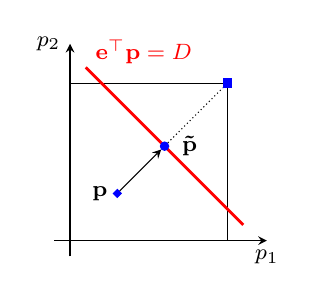
\begin{tikzpicture}[x=2cm,y=2cm]
        % X Axis
        \draw[black,-stealth] (-0.1, 0.0) -- (1.25, 0.0);
        \node[below] at (1.25, 0.0) {\footnotesize $p_{1}$};
        % Y axis
        \draw[black,-stealth] (0.0, -0.1) -- (0.0, 1.25);
        \node[left] at (0.0, 1.25) {\footnotesize $p_{2}$};
        
        % Unit hypercube
        \draw[black] (0,0) -- (0, 1) -- (1,1) -- (1,0) -- cycle;
        
        % Power balance constraint
        \draw[red,line width=1pt] (0.1, 1.1) -- (1.1, 0.1);
        \node[right, color=red] at (0.1, 1.2) {\footnotesize $\mathbf{e}^{\top}\pg = D$};
        
        % Max output
        \node[draw=blue, fill=blue, inner sep=0pt,minimum size=3pt] (p_bar) at (1.00, 1.00) {};
        % Prediction
        \node[diamond,draw=blue, fill=blue, inner sep=0pt,minimum size=3pt] (p_hat) at (0.30, 0.30) {};
        \node[left] at (0.3, 0.3) {\footnotesize $\pg$};
        % Feasible point
        \node[circle,draw=blue, fill=blue, inner sep=0pt,minimum size=3pt] (p_til) at (0.6, 0.6) {};
        \node[right] at (0.65, 0.6) {\footnotesize $\mathbf{{\tilde{p}}}$};
        
        % Proportional response visual
        \draw[black,-stealth] (p_hat) -- (p_til);
        \draw[black,densely dotted] (p_til) -- (p_bar);
    \end{tikzpicture}}
    \hfill
    \resizebox{0.42\columnwidth}{!}{
    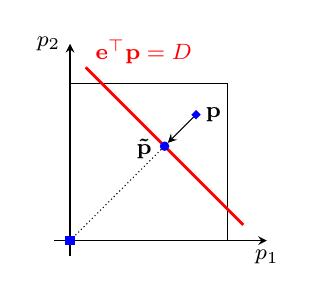
\begin{tikzpicture}[x=2cm,y=2cm]
        % X Axis
        \draw[black,-stealth] (-0.1, 0.0) -- (1.25, 0.0);
        \node[below] at (1.25, 0.0) {\footnotesize $p_{1}$};
        % Y axis
        \draw[black,-stealth] (0.0, -0.1) -- (0.0, 1.25);
        \node[left] at (0.0, 1.25) {\footnotesize $p_{2}$};
        
        % Unit hypercube
        \draw[black] (0,0) -- (0, 1) -- (1,1) -- (1,0) -- cycle;
        
        % Power balance constraint
        \draw[red,line width=1pt] (0.1, 1.1) -- (1.1, 0.1);
        \node[right, color=red] at (0.1, 1.2) {\footnotesize $\mathbf{e}^{\top}\pg = D$};
        
        % Min output
        \node[draw=blue, fill=blue, inner sep=0pt,minimum size=3pt] (p_bar) at (0.00, 0.00) {};
        % Prediction
        \node[diamond,draw=blue, fill=blue, inner sep=0pt,minimum size=3pt] (p_hat) at (0.80, 0.80) {};
        \node[right] at (0.8, 0.8) {\footnotesize $\pg$};
        % Feasible point
        \node[circle,draw=blue, fill=blue, inner sep=0pt,minimum size=3pt] (p_til) at (0.6, 0.6) {};
        \node[left] at (0.58, 0.58) {\footnotesize $\mathbf{{\tilde{p}}}$};
        
        % Proportional response visual
        \draw[black,-stealth] (p_hat) -- (p_til);
        \draw[black,densely dotted] (p_til) -- (p_bar);
    \end{tikzpicture}}
    \hfill\\
    \caption{%
        Illustration of the power balance layer with input $\pg$ and output $\mathbf{\tilde{p}}$.
        Left: $\mathbf{e}^{\top}\pg \, {<} \, D$ (energy shortage) and generators' dispatches are increased.
        Right: $\mathbf{e}^{\top}\pg \, {>} \, D$ (energy surplus) and generators' dispatches are decreased.
    }
    \label{fig:feasibility_layer:hypersimplex}
\end{figure}


the output is given by:

\begin{align*}
    \mathcal{P}(\pg) &= \begin{cases}
        (1 - \eta^{\uparrow}) \pg + \eta^{\uparrow} \pgmax & \text{if } \mathbf{e}^{\top} \pg < \mathbf{e}^{\top} \pd \\
        (1 - \eta^{\downarrow}) \pg + \eta^{\downarrow} \mathbf{0} & \text{if } \mathbf{e}^{\top} \pg > \mathbf{e}^{\top} \pd
    \end{cases} \\
    \eta^{\uparrow} &= \frac{\mathbf{e}^{\top} \pd - \mathbf{e}^{\top} \pg}{\mathbf{e}^{\top} \pgmax - \mathbf{e}^{\top} \pg}, \quad
    \eta^{\downarrow} = \frac{\mathbf{e}^{\top} \pg - \mathbf{e}^{\top} \pd}{\mathbf{e}^{\top} \pg - \mathbf{e}^{\top} \mathbf{0}}
\end{align*}

The reserve repair layer $\mathcal{R}$ takes as input an initial dispatch vector $\pg \in \hypersimplex{D}$ and outputs a dispatch vector $\mathbf{\tilde{p}}$ that also satisfies the reserve requirement.

\begin{figure}[ht]
    \centering
    \resizebox{0.6\columnwidth}{!}{
    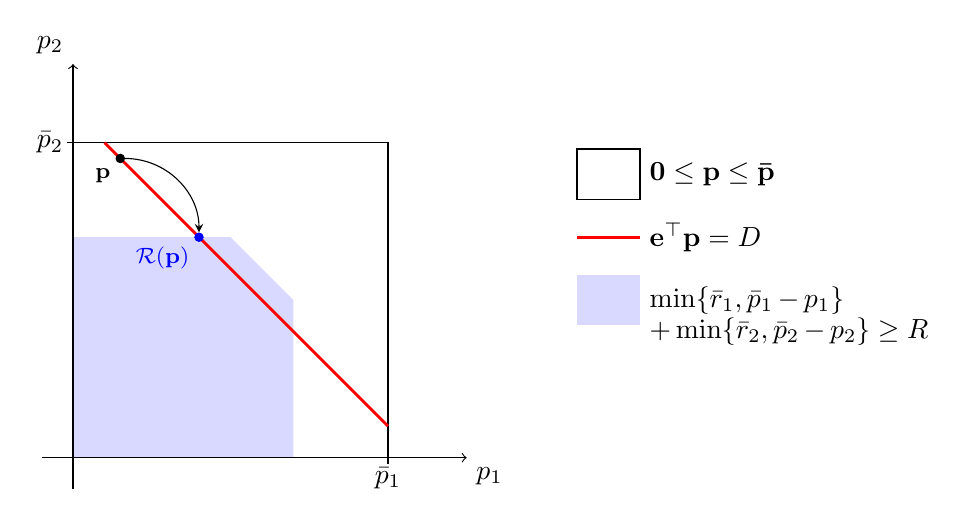
\begin{tikzpicture}[x=4cm,y=4cm]
        % X Axis
        \draw[black,->] (-0.1, 0.0) -- (1.25, 0.0);
        \node[below right] at (1.25, 0.0) {$p_{1}$};
            \draw[black] (1, -0.02) -- (1, 0.02);
            \node[below] at (1, 0.0) {$\bar{p}_{1}$};
        
        % Y axis
        \draw[black,->] (0.0, -0.1) -- (0.0, 1.25);
        \node[above left] at (0.0, 1.25) {$p_{2}$};
            \draw[black] (-0.02, 1) -- (+0.02, 1);
            \node[left] at (0, 1) {$\bar{p}_{2}$};
            
        % Reserve feasibility domain
        \fill[blue!50!white, fill opacity=0.3] (0,0) -- (0,0.7) -- (0.5, 0.7) -- (0.7, 0.5) -- (0.7, 0.0) -- cycle;
        
        % Domain of p1, p2
        \draw[black] (0,0) -- (0, 1) -- (1,1) -- (1,0) -- cycle;
        
        % Power balance constraint
        \draw[red,line width=1pt] (0.1, 1.0) -- (1.0, 0.1);
        
        % Infeasible prediction
        \node[circle,draw=black, fill=black, inner sep=0pt,minimum size=3pt] (phat_a) at (0.15, 0.95) {};
        \node[below left] at (0.15, 0.95) {\footnotesize $\pg$};
        
        % Feasible points of interest
        \node[circle,draw=blue, fill=blue, inner sep=0pt,minimum size=3pt] (pfeas1) at (0.4, 0.7) {};
        \node[below left, blue] at (0.4, 0.7) {\footnotesize $\mathcal{R}(\pg)$};
        
        \draw[-stealth] (phat_a.east) to [out=0,in=90] (pfeas1.north);
        
        % Legend
            % Domain of pg
            \draw[black] (1.6, 0.98) -- (1.8, 0.98) -- (1.8, 0.82) -- (1.6, 0.82) -- cycle;
            \node[right] at (1.8, 0.9) {$\mathbf{0} \leq \pg \leq \mathbf{\bar{p}}$};
            % Power Balance
            \draw[red, line width=1pt] (1.6, 0.7) -- (1.8, 0.7);
            \node[right] at (1.8, 0.7) {$\mathbf{e}^{\top} \pg = D$};
            % Reserve feasibility
            \fill[blue!50!white, fill opacity=0.3] (1.6, 0.58) -- (1.8, 0.58) -- (1.8, 0.42) -- (1.6, 0.42) -- cycle;
            \node[right] at (1.8, 0.5) {$\min\{\bar{r}_{1}, \bar{p}_{1} \, {-} \, p_{1}\}$};
            \node[right] at (1.8, 0.4) {$+\min\{\bar{r}_{2}, \bar{p}_{2} \, {-} \, p_{2}\} \geq R$};
    \end{tikzpicture}
    }
    \caption{Illustration of the reserve feasibility layer for $\mathbf{\bar{p}} {=} (1, 1)$, $\mathbf{\bar{r}}{=}(0.5, 0.5)$, $D {=} 1.1$, $R{=}0.8$ and the initial prediction $\pg {=} (0.15, 0.95)$. The recovered feasible dispatch is $\mathbf{\tilde{p}} {=} (0.4, 0.7)$.}
    \label{fig:feasibility_recovery:reserve}
\end{figure}


the output is given by the following algorithm:
\begin{algorithm}[t]
    \caption{Reserve Repair Layer}
    \label{alg:FFR:reserves}
    \begin{algorithmic}[1]
        \REQUIRE Initial prediction $\pg \in \hypersimplex{D}$, maximum limits $\mathbf{\bar{p}}, \mathbf{\bar{r}}$, reserve requirement $R$
        \STATE $\Delta_{R} \gets R - \sum_{g} \min \{ \bar{r}_{g}, \bar{p}_{g} - p_{g} \}$
        \STATE $\mathcal{G}^{\uparrow} \gets \left\{ g \ \middle| \ p_{g} \leq \bar{p}_{g} - \bar{r}_{g} \right\}$
        \STATE $\mathcal{G}^{\downarrow} \gets \left\{ g \ \middle| \  p_{g} > \bar{p}_{g} - \bar{r}_{g} \right\}$
        \STATE $\Delta^{\uparrow} \gets \sum_{g \in \mathcal{G}^{\uparrow}} (\bar{p}_{g} - \bar{r}_{g}) - p_{g}$
        \STATE $\Delta^{\downarrow} \gets \sum_{g \in \mathcal{G}^{\downarrow}} p_{g} - (\bar{p}_{g} - \bar{r}_{g})$
        \STATE $\Delta \gets \max(0, \min(\Delta_{R}, \Delta^{\uparrow}, \Delta^{\downarrow}))$
        \STATE $\alpha^{\uparrow} \gets \Delta / \Delta^{\uparrow}$, $\alpha^{\downarrow} \gets \Delta / \Delta^{\downarrow}$, \label{alg:FFR:proportional_response_weigths}
        \STATE Energy dispatch adjustment
            \begin{align*}
                \tilde{p}_{g} &= \left\{
                    \begin{array}{ll}
                        (1 - \alpha^{\uparrow}) p_{g} + \alpha^{\uparrow} (\bar{p}_{g} - \bar{r}_{g}) & \forall g \in \mathcal{G}^{\uparrow} \\
                        (1 - \alpha^{\downarrow}) p_{g} + \alpha^{\downarrow} (\bar{p}_{g} - \bar{r}_{g}) & \forall g \in \mathcal{G}^{\downarrow}
                    \end{array}
                \right.
            \end{align*}
            \label{alg:FFR:proportional_response}
        \STATE \textbf{return} $\mathcal{R}(\pg) = \mathbf{\tilde{p}}$
    \end{algorithmic}
\end{algorithm}



\section*{Experimental results}
\subsection*{Dataset}
The 6 datasets are derived from reference test cases in the PGLib library.
\begin{table}[ht]
\centering
\renewcommand{\arraystretch}{0.9}
\begin{tabular}{|l|c|c|c|l|}
\hline
\textbf{System Name} & \textbf{Buses ($|\mathcal{N}|$)} & \textbf{Generators ($|\mathcal{G}|$)} & \textbf{Branches ($|\mathcal{E}|$)} & \textbf{Type} \\
\hline
ieee300 & 300 & 69 & 411 & Academic \\
\hline
pegase1k & 1,354 & 260 & 1,991 & Realistic \\
\hline
rte6470 & 6,470 & 761 & 9,005 & Real (French Grid) \\
\hline
pegase9k & 9,241 & 1,445 & 16,049 & Realistic \\
\hline
pegase13k & 13,659 & 4,092 & 20,467 & Realistic \\
\hline
goc30k & 30,000 & 3,526 & 35,393 & Synthetic (Large Scale) \\
\hline
\end{tabular}
\end{table}
The authors generated many datapoints by perturbing the reference cases. They created two categories of datasets: ED (Economic Dispatch without reserves) and ED-R (with reserves).

The ground truth solutions were computed using the Gurobi optimizer.

\subsection*{Implementation details}
% loss functions
The loss functions for supervised learning and self-supervised learning were:
\[\mathcal{L}^{SL}(\hat{p}, p^*) = \underbrace{\frac{1}{|\mathcal{G}|} ||\hat{p} - p^*||_1}_{\text{MAE of Dispatch}} + \underbrace{\mu M_{th} ||\xi_{th}(\hat{p})||}_{\text{Thermal Constraints}} + \underbrace{\lambda \psi(\hat{p})}_{\text{Hard Constraints}}\]
\[\mathcal{L}^{SSL}(p^*) = \underbrace{c(p^*)}_{\text{Generation Cost}} + \underbrace{M_{th} \xi_{th}(p^*)}_{\text{Thermal Penalties}} + \underbrace{\lambda \psi(\hat{p})}_{\text{Hard Constraints}}\]
\[\psi(\hat{p}) = M_{pb}|e^T\boldsymbol{d} - e^T\hat{p}| + M_{r}\xi_{r}(\hat{p})\]
where the hyperparameters were: $M_{th} = 1500$, $M_{pb} = 3500$, $M_{r} = 1100$.

The models are simple Feed Forward Neural Networks with a sigmoid activation function and the repair layers. The dataset was split into 40000/5000/5000 for training/validation/test. The optimization was done using the Adam optimizer. The learning rate was reduced by a factor of 10 when the validation loss stopped improving for 10 consecutive epochs. The training was stopped when the validation loss stopped improving for 20 consecutive epochs. The hyperparameters were optimized using grid search.

\subsection*{Results}
The results have shown that the E2ELR model performed better than the other models in terms of accuracy on every dataset. The E2ELR models also took around the same time to infer a solution as a DNN and much faster than the Gurobi optimizer.


\bibliographystyle{ieeetr}
\bibliography{refs}

\end{document}